\section{Study Design}\label{sec:study_design}

We decided to evaluate our prototype in a semi-naturalistic field-study, comparing it against similar methods, capable of recording \CSE for individual segments of a larger route.
This section describes how we went about designing this study.

\subsection{Recording Methods}\label{subsec:recording_methods}

Our method using the “LikertShift” device works by recording its currently selected value, whenever we receive a new GPS location.
Thus, a selected value remains valid until the users selects a new one, and we receive their next GPS location, so a new rating gets recorded whenever they notice a change in their subjective experience and remains valid, onwards from that point in time, until they adjust the rating again.
This allows users to choose a rating frequency they consider appropriate by themselves.

We selected two methods from our survey of the related work we regard as suitable to compare against our method and adjusted them, to allow for a fair comparison.
The first one, referred to as “Audio Recording” from now on, is taken from the work of \citetext{evaluation_models_for_cyclists_perception}{Yamanaka et al.}, who captured audio data while cycling and required participants to rate pre-defined route-segments using multiple measures on scales from 1 to 5.
We adjusted it to only used one measure and also let participants perform ratings on arbitrary route segments, in contrast to pre-defined ones.
The second method, referred to as “Mapping” is the one proposed by \citetext{using_mental_mapping}{Manton et al.}, who let participants color code segments of a previously driven route, based on their risk assessment.
In our study, we provided participants with a printed map, picturing the route they drove and let them divide it into multiple segments themselves, assigning a numerical rating to each segment, instead of color coding it.

\subsubsection*{Choosing a Measure}

We had to take great care to select a suitable measure, so we could compare the data collected by different participants and the different methods against each other.
This is inherently difficult, as cyclists' subjective experiences are arguably very subjective and will thus vary drastically from participant to participant.

As mentioned in the introduction to \autoref{sec:related_work}, most works rely on risk/safety and stress/comfort measures to quantify \CSE.
The advantage of using risk/safety would be its independence from many external factors and high dependence on the chosen route.
Constructing a route with highly varying risk factors would be comparatively easy, but deliberately placing participants in high-risk environments would be extremely unethical, which led us to quickly dismiss that approach.
Letting participants rate their comfort level or travel satisfaction comes with its own set of challenges though.
Overall comfort level depends on a lot of actors, such as participants initial mood, their experience in riding a bicycle, but also external factors such as weather, traffic, or surrounding scenery of the route.
To be able to properly compare our recorded datasets against each other, we needed to find a way to eliminate as many of these factors as possible.

As findings by \citetext{thinking_aloud_on_the_road}{McIlroy et al.} revealed the high impact of road surface quality on cyclists overall comfort and satisfaction with their travel, we decided to limit our measure to this, using the metric of “Travel satisfaction, based on the road” as the \CSE measure that participants have to use to rate segments of the route.
We carefully explained this metric to each participant before conducting the study, instructing them on what should (road condition, road type, available space, slope of the road, etc.) and should not (general mood, current traffic situation, route scenery, etc.) affect their ratings.
Ratings were to be performed on a Likert scale from 1 to 5, denoting high dissatisfaction and high satisfaction, respectively.
This measure should exert a similar mental demand on participants, as they still need to feel out their comfort level, while increasing data quality, allowing us to perform quantitative comparisons of the different methods used.
\subsection{Route Selection}

If each participant was to evaluate all three methods after each other on the same route, we would expect to see an increase in accuracy for subsequent route traversals, as by that point the route is already known.
Thus, we constructed three different routes and balanced route orders, method orders as well as the number of routes per method in our study.
We chose each route to take $\sim\SI{10}{min}$ to complete for an average cyclist and ensured it contained a multitude of different road types and crossings.
As we wanted to conduct the study in a single session per participant, at our university campus, we were limited by the available traffic infrastructure in the immediate vicinity and also had to put all start and endpoints in the approximate same location.

\begin{table}[!htb]
    \footnotesize
    \centering
    \begin{tabular}{c|c|ccccc|c}
        \multirow{2}{*}{Name} & \multirow{2}{2.4em}{Total\newline} & \multicolumn{5}{c|}{Road Type} & \multirow{2}{4.7em}{Number of\newline}\\
        \cline{3-7}
        &&&&&&&\\[-1em]
        & Length & Road & Bike Path & Mixed Path & Pedestrian Way & Other & Crossings\\[0.15em]
        \hline
        &&&&&&&\\[-0.8em]
        North & \SI{2589}{m} &  \SI{191}{m} & \SI{480}{m} & \SI{1135}{m} & \SI{359}{m} & \SI{424}{m} & 13\\[0.3em]
        East  & \SI{2007}{m} &  \SI{853}{m} & \SI{465}{m} &  \SI{173}{m} & \SI{181}{m} & \SI{335}{m} & 9\\[0.3em]
        South & \SI{2289}{m} & \SI{1152}{m} & \SI{677}{m} &  \SI{116}{m} &  \SI{47}{m} & \SI{297}{m} & 9\\
    \end{tabular}
    \caption{Overview of the study routes}
    \label{table:routes_overview}
\end{table}

\noindent
\autoref{table:routes_overview} shows the total lengths of the routes, as well as an overview of the different road types and number of crossings per route.
Each route is named according to the direction it starts towards.
The study was conducted at the Campus Adlershof\footnoteurl{https://www.hu-berlin.de/en/about/campus/adlershof} of the Humboldt University of Berlin, located in a mixed-use area outside the city center.
Notably, the roads participants had to drive on were mostly side-roads with very little traffic and therefore received a more positive rating than one might expect.
We also opted to use existing cycling infrastructure wherever possible, only evading to drive on the road when no such infrastructure was available.
Furthermore, mixed-paths refer to areas mainly intended to be used by pedestrians that are spacious enough to allow for cycling at low speeds.

\begin{figure}[!htb]
    \centering
    \begin{minipage}{.5\textwidth}
        \centering
        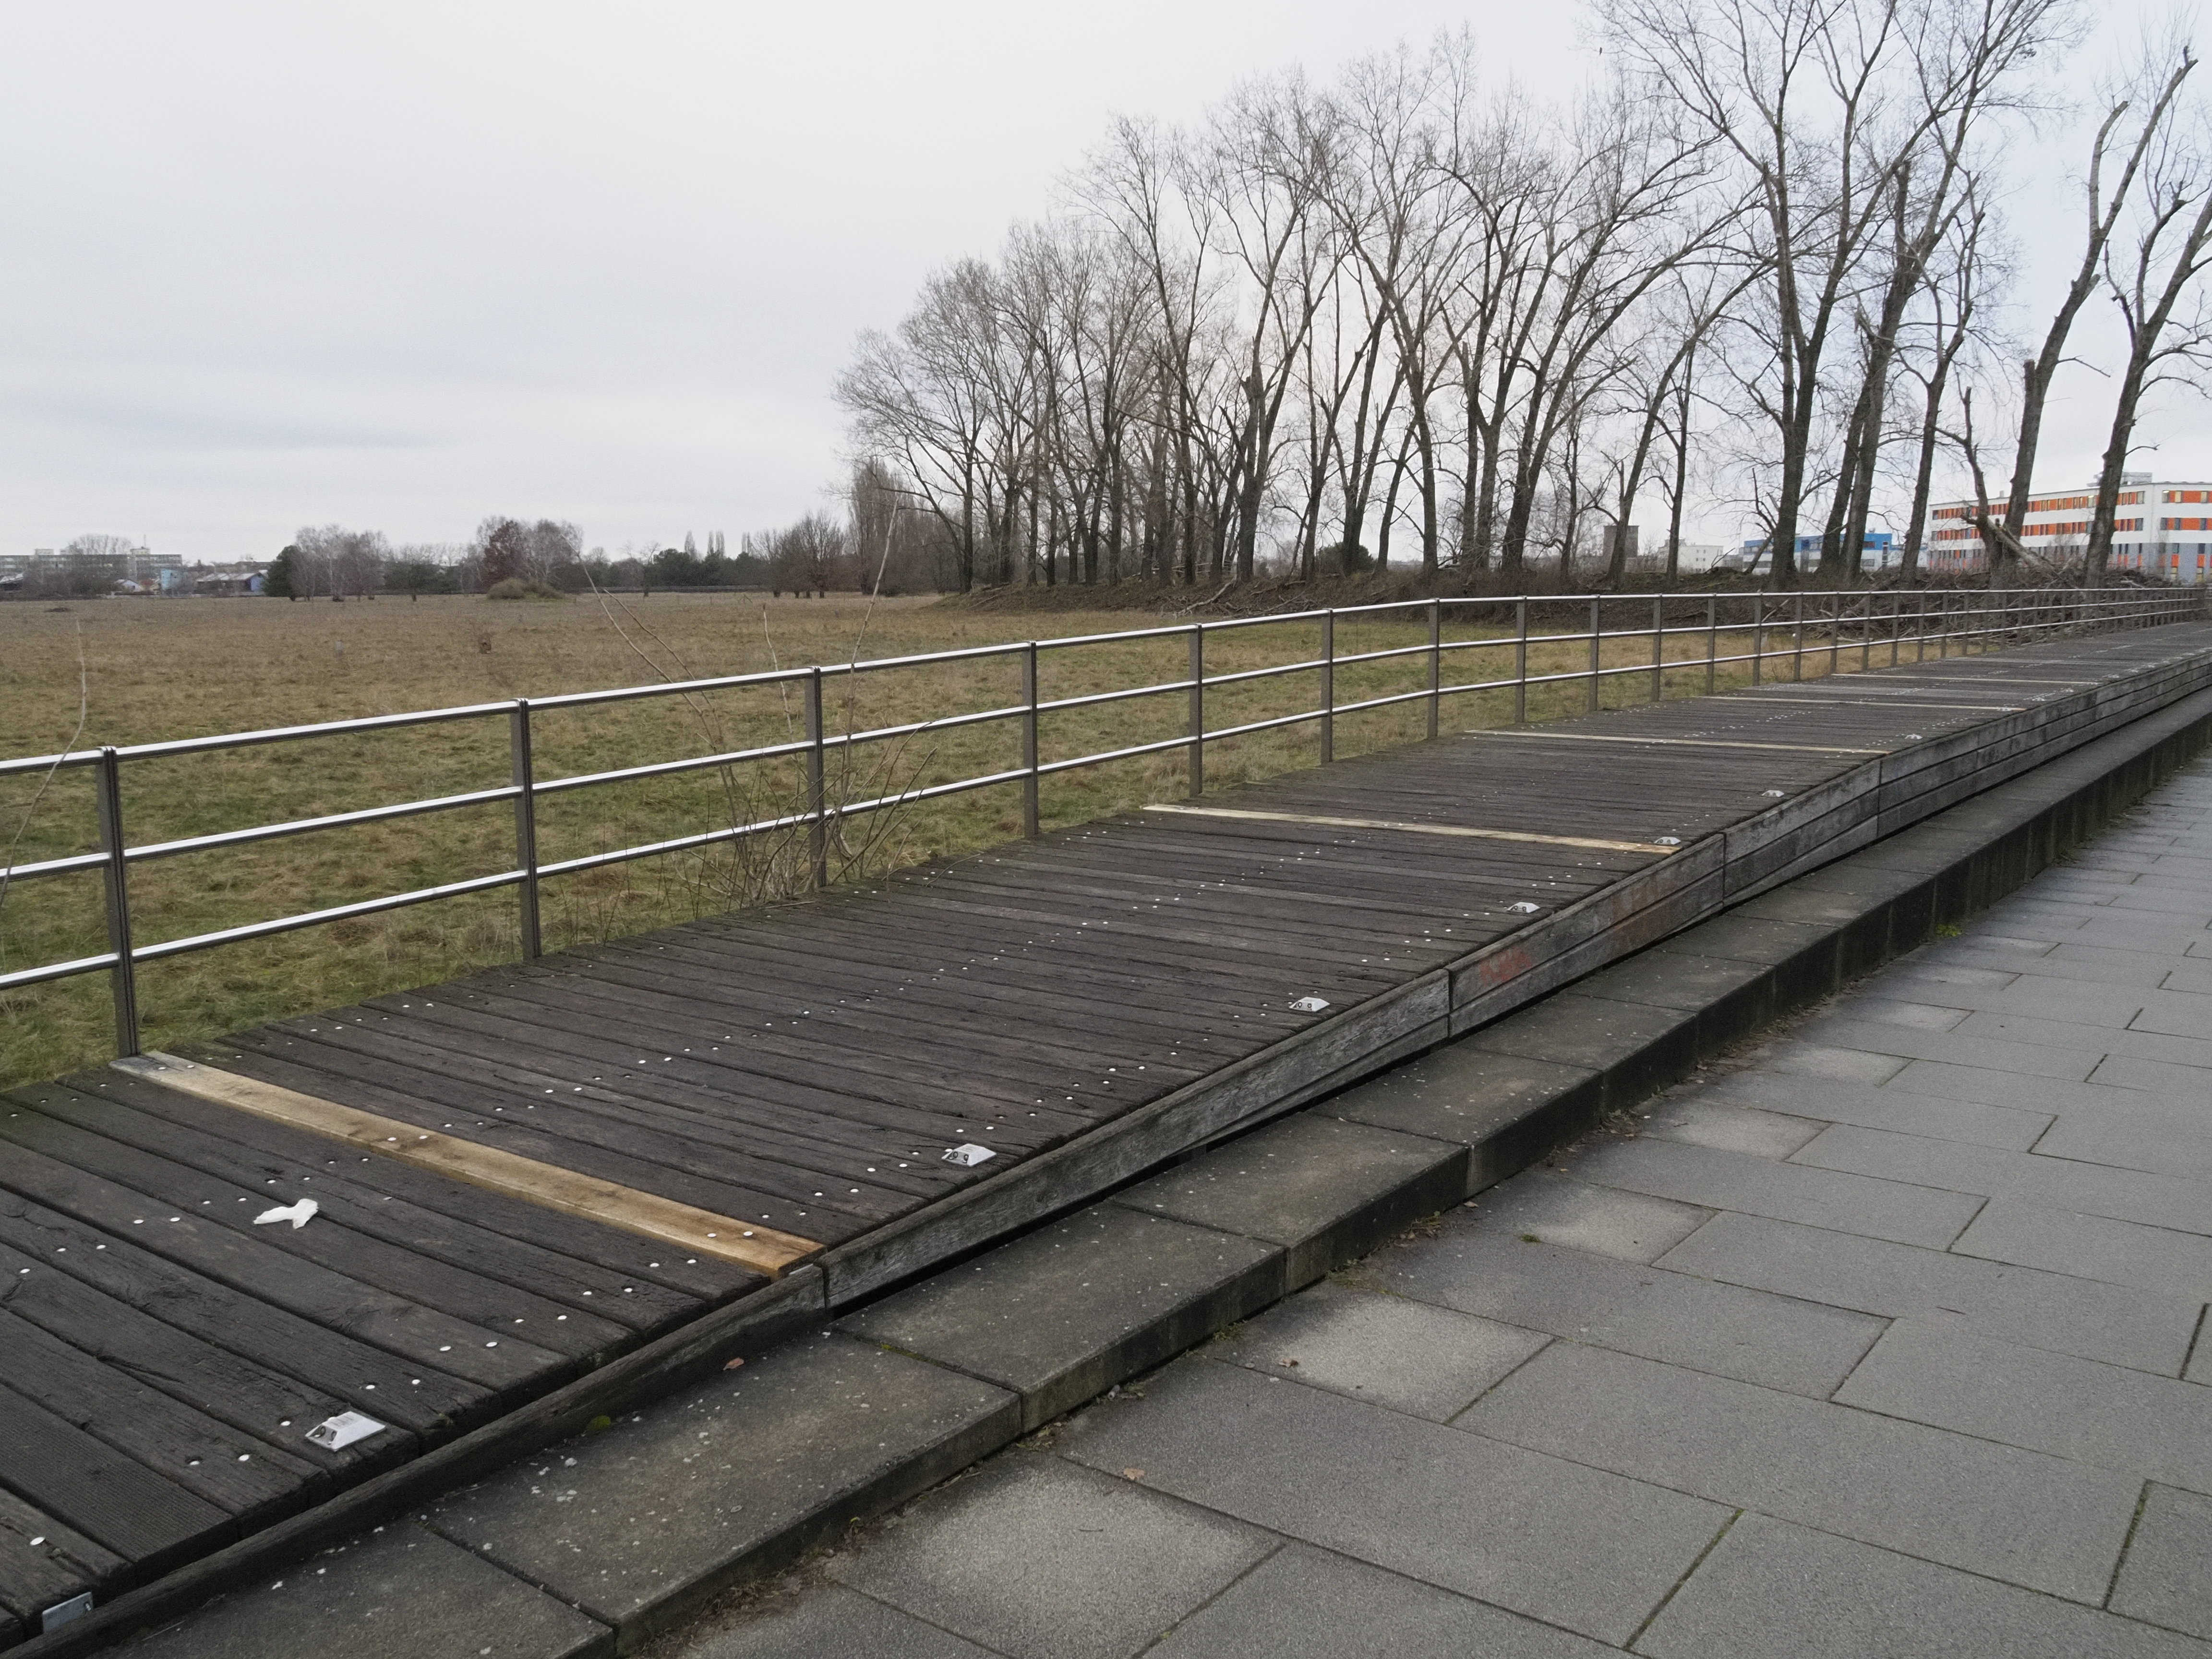
\includegraphics[width=.9333\linewidth]{images/wood_planks_path.jpg}
        \caption{Elevated path (wood planks)}
        \label{fig:wood_planks}
    \end{minipage}%
    \begin{minipage}{.5\textwidth}
        \centering
        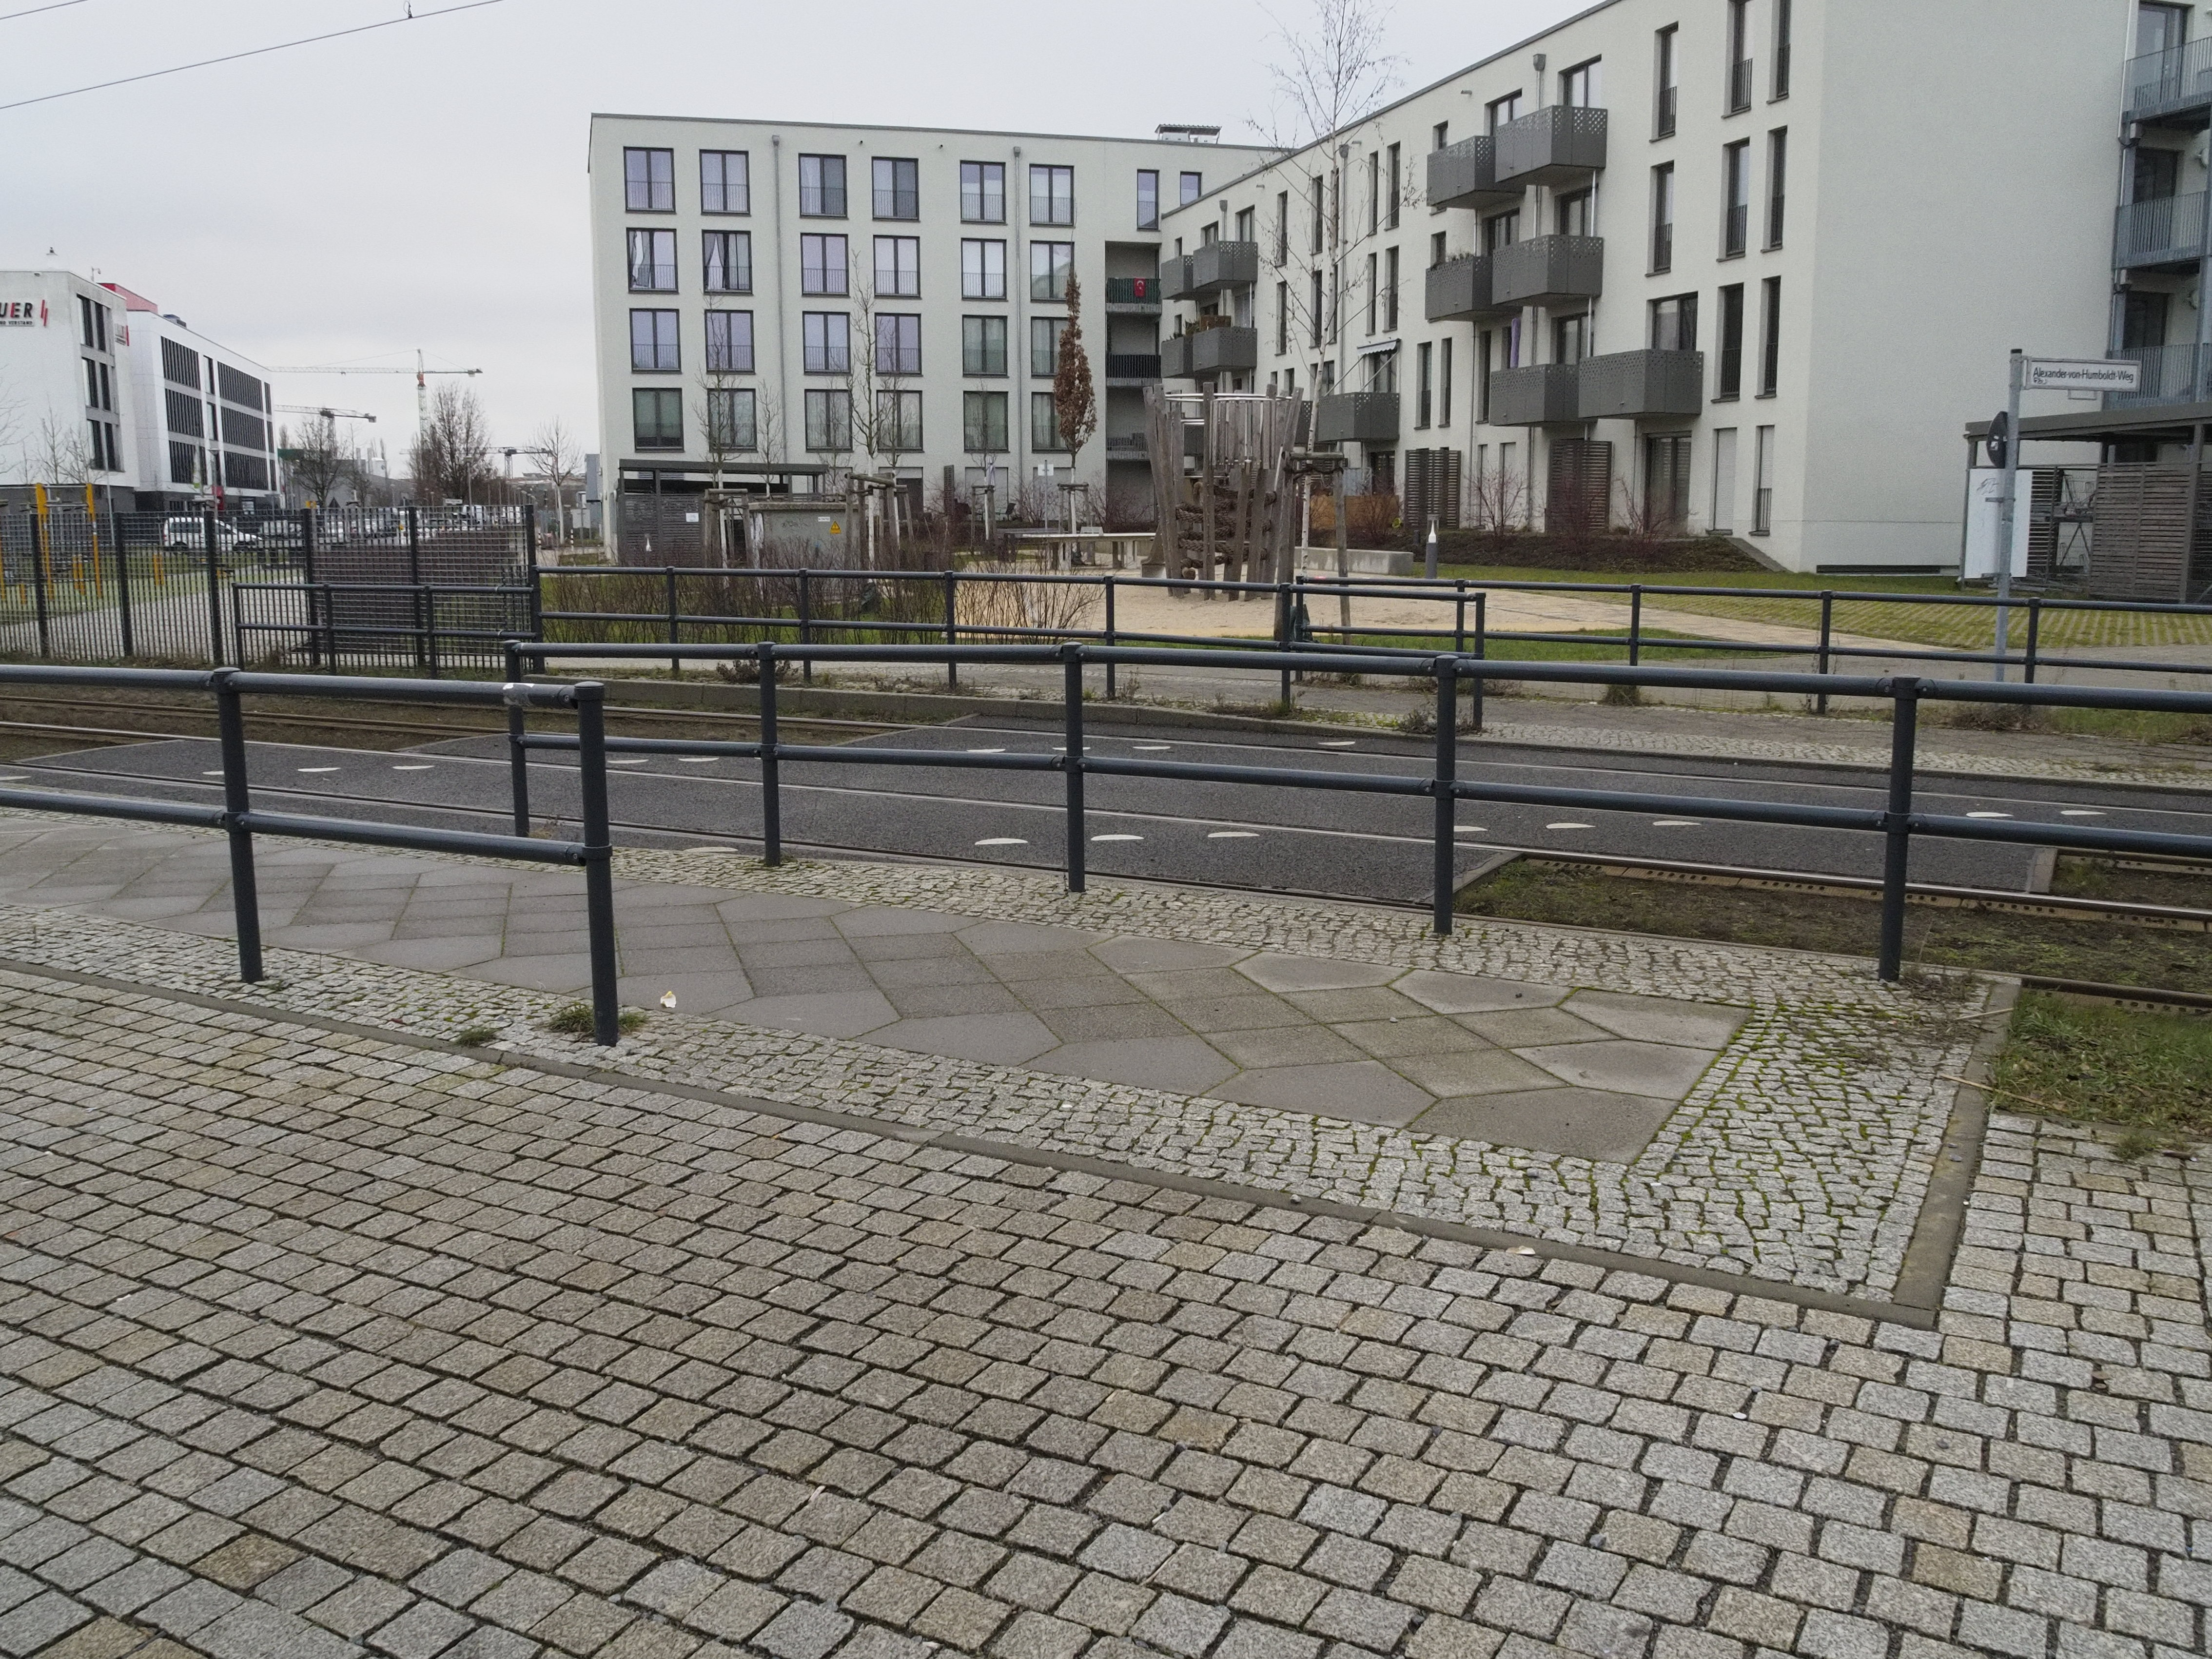
\includegraphics[width=.9333\linewidth]{images/tram_crossing.jpg}
        \caption{Tram crossing}
        \label{fig:tram_crossing}
    \end{minipage}
\end{figure}

\bigbreak\noindent
We also chose each route to contain at least one section that particularly stands out from the rest of the route.
For the “North” route this was an elevated wooden path (\autoref{fig:wood_planks}), as well as an awkward tram crossing (\autoref{fig:tram_crossing}).
The “East” route contained the objectively worst terrain of our study, a very rugged field participants had to traverse (\autoref{fig:field_east}).
The “South” route also featured an “off-road” section, traversing a lawn next to a building, this one was noticeably more flat though (\autoref{fig:field_south}).
The “East” and “South” routes also both featured different sections blocked by the same construction site (\autoref{fig:construction_site}), where participants had to result to driving on pedestrian ways.

\begin{figure}[!htb]
    \centering
    \begin{minipage}{.3333\textwidth}
        \centering
        \includegraphics[width=.9\linewidth]{images/field_east_route.jpg}
        \caption{Rugged field}
        \label{fig:field_east}
    \end{minipage}%
    \begin{minipage}{.3333\textwidth}
        \centering
        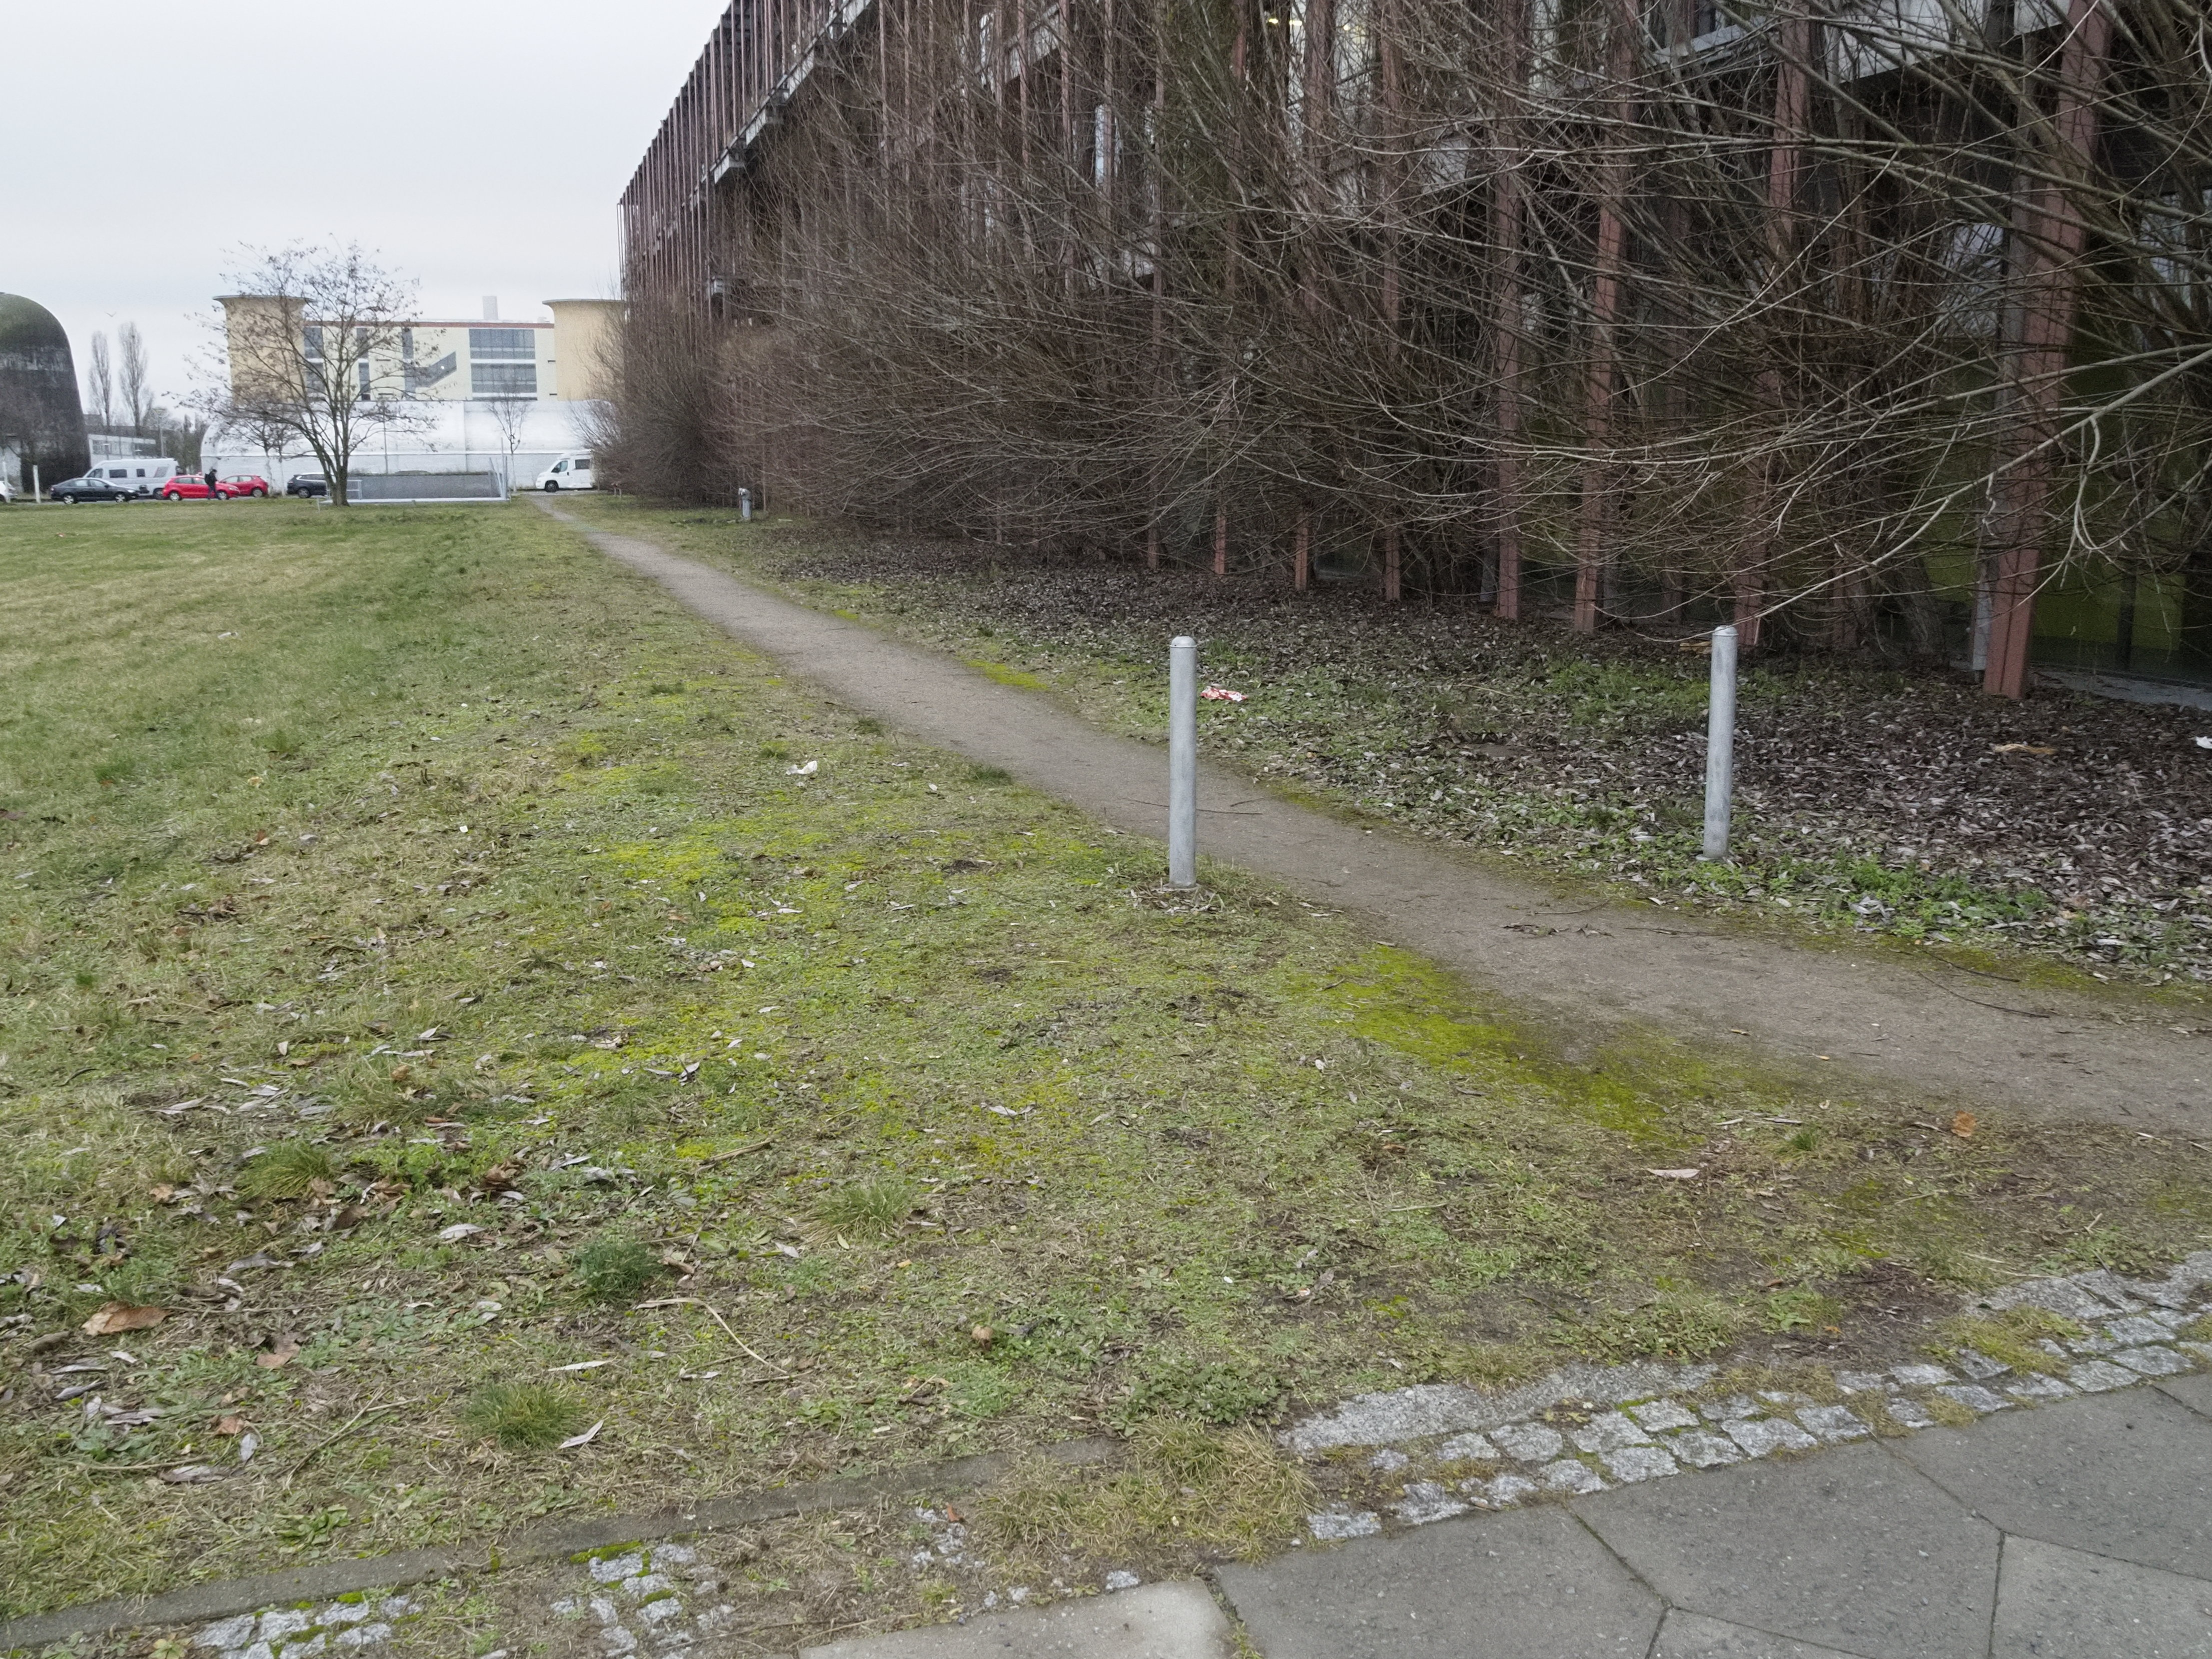
\includegraphics[width=.9\linewidth]{images/field_south_route.jpg}
        \caption{Flat lawn}
        \label{fig:field_south}
    \end{minipage}%
    \begin{minipage}{.3333\textwidth}
        \centering
        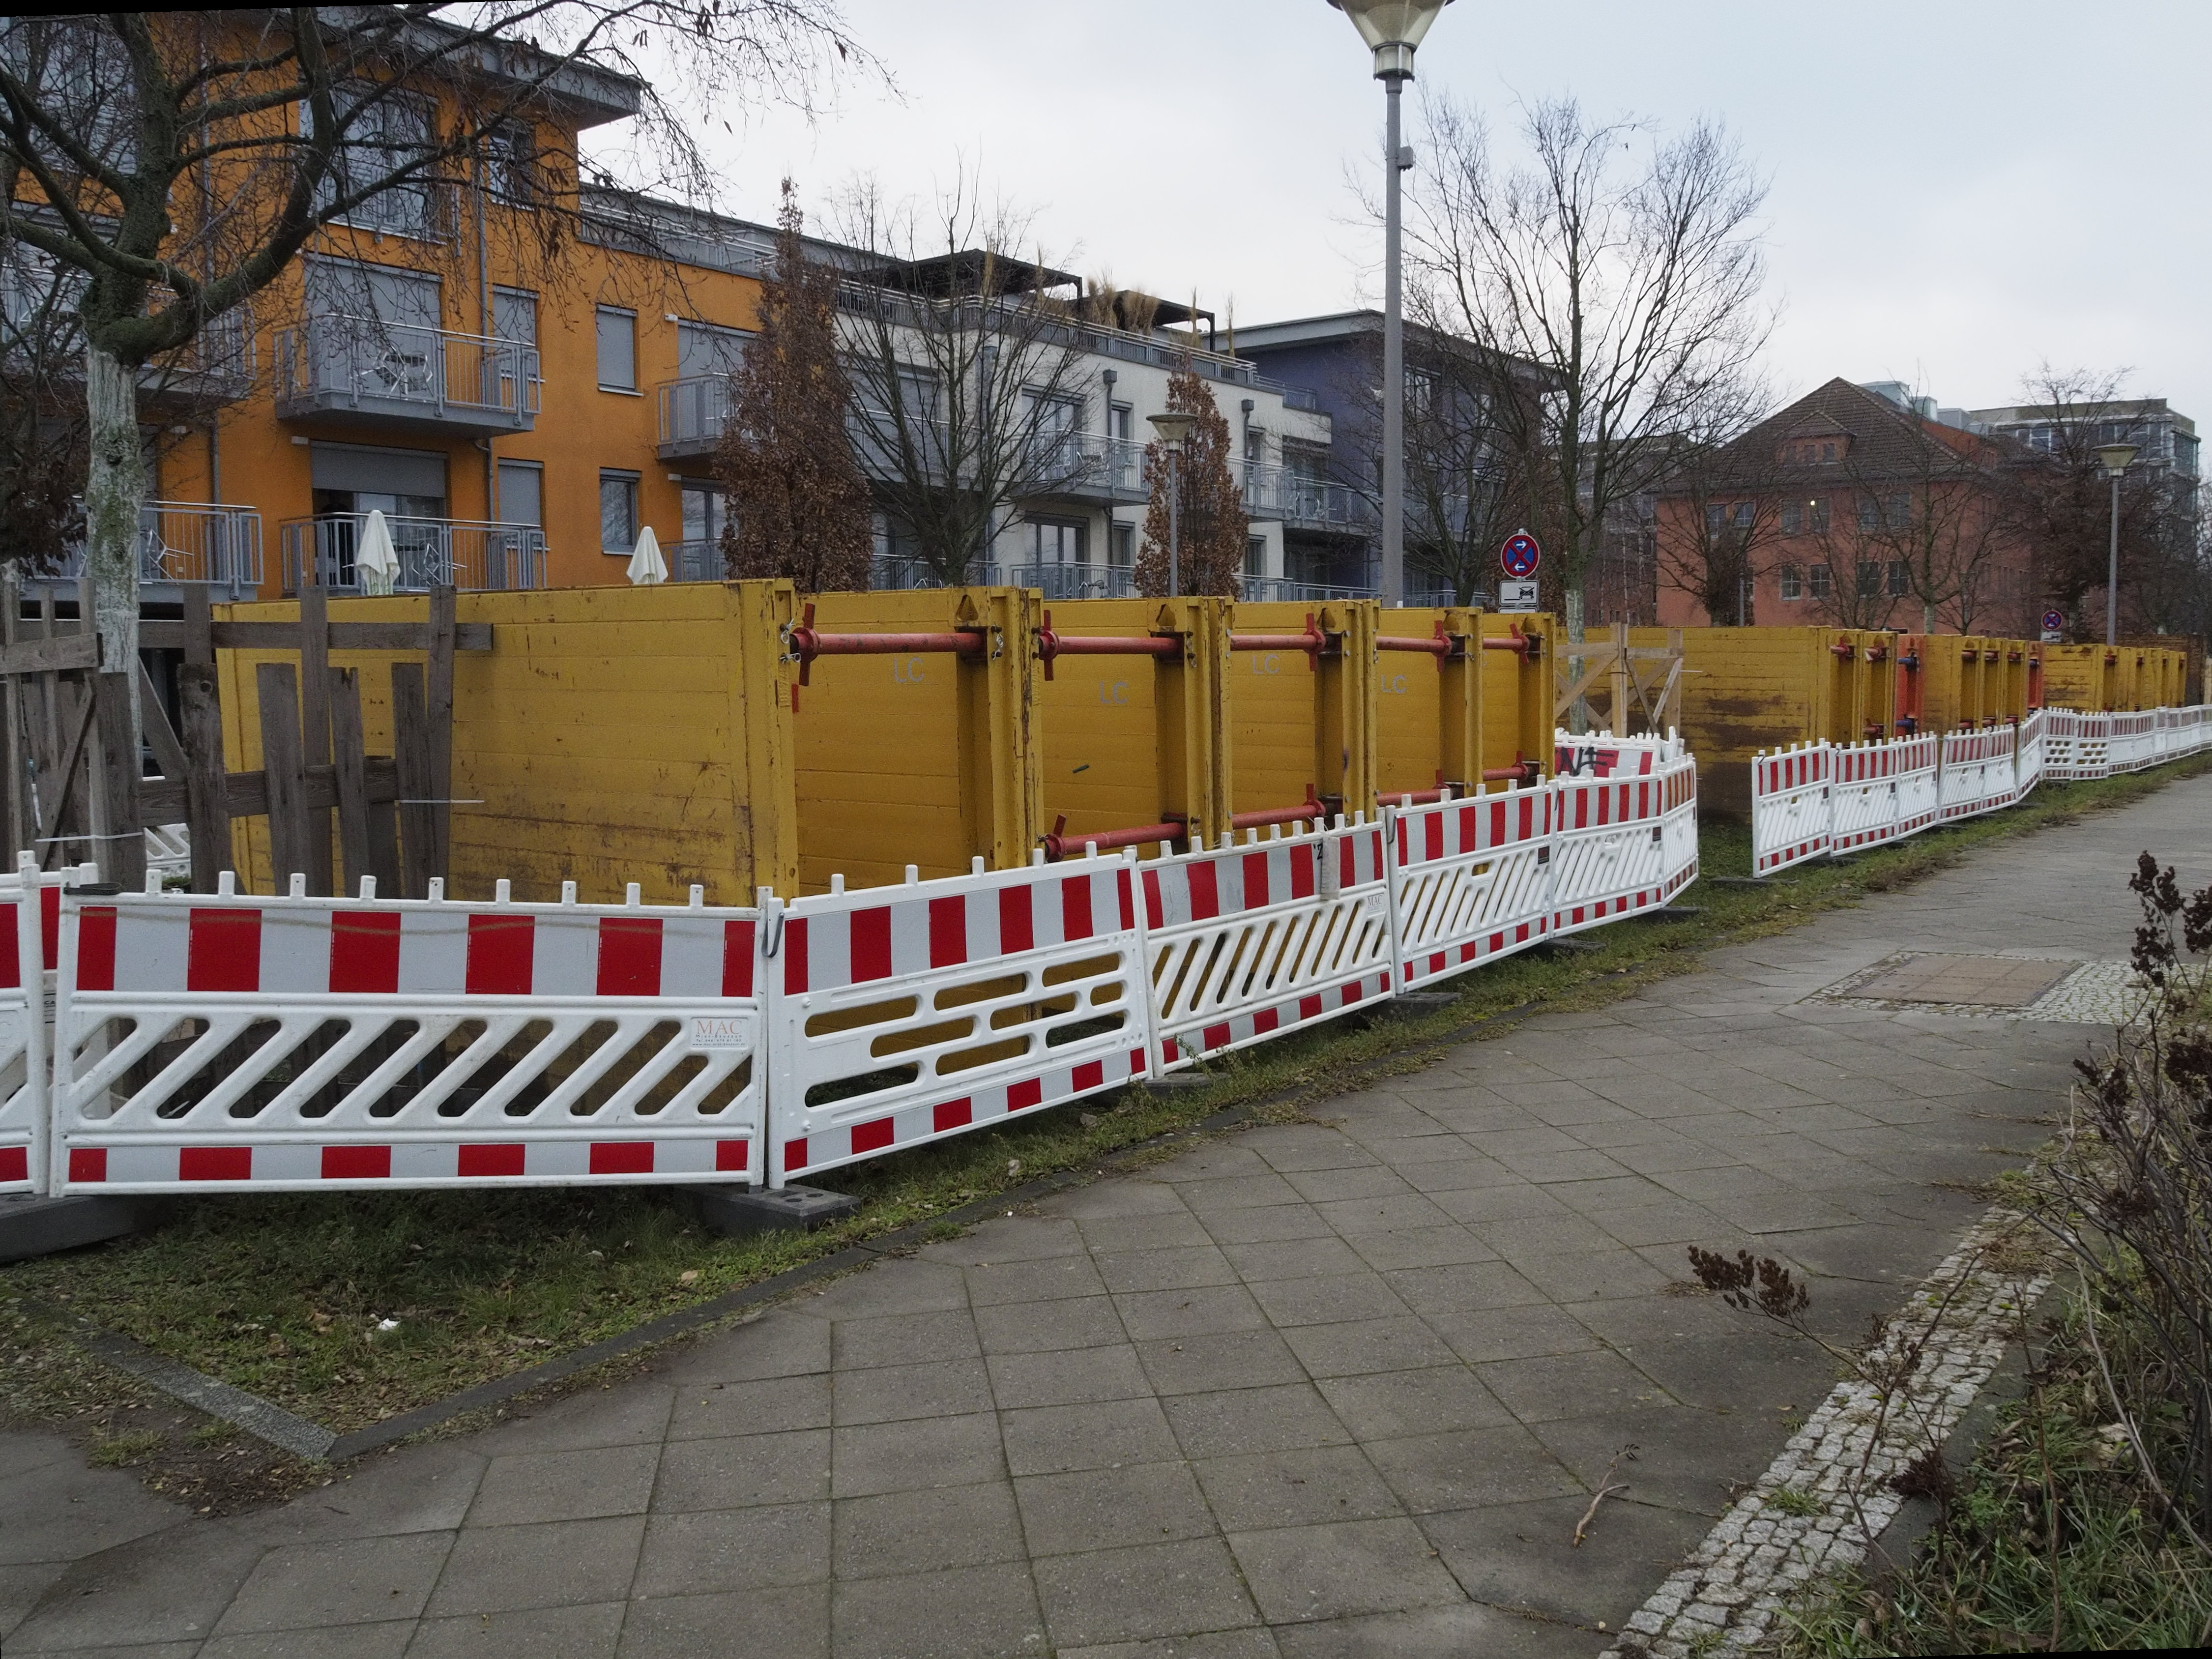
\includegraphics[width=.9\linewidth]{images/construction_site.jpg}
        \caption{Construction site}
        \label{fig:construction_site}
    \end{minipage}
\end{figure}

\subsection{Data Collection}\label{subsec:data_collection}

All data was collected using the \likertshift app acting as a frontend for our prototype, as described in \autoref{subsec:frontend_design} and the \audiorecording and \mapping methods were added to it.
\audiorecording is implemented by using the smartphones internal microphone to record an audio track while cycling.
The recorded audio will then be added to the recording data as a lossless \texttt{FLAC} file.
For the \mapping method, we only recorded location and time information in the app.
The actual ratings were performed retrospectively on a piece of paper.
After resetting the app at the end of each study participation, we simply wrote down the participants ID on said piece of paper, to be able to match it with the recorded data later on.
This is described in more detail in \autoref{subsec:preprocessing}.

\subsubsection{Questionnaires}

In addition to this quantitative data, we also used two questionnaires, the \citetext{nasa_tlx}{NASA TLX} and the \citetext{ueq+}{UEQ+} (a modular extension of the commonly used \citetext{ueq}{UEQ}) to obtain qualitative data, regarding differences between the recording methods used.
Participants were asked to fill in these questionnaires right after they finished rating a route with each method.
We made sure participants understood that both questionnaires only concerned the respective method used to rate their subjective experience during cycling, but not the act of cycling itself.
For the \citetextnoref{ueq+}{UEQ+}, we selected the \textit{Attractiveness}, \textit{Efficiency}, \textit{Intuitive Use}, \textit{Hardware Security} and \textit{Social Acceptance} scales and slightly adjusted some questions wordings, as the \citetextnoref{ueq+}{UEQ+} is usually used to evaluate the user experience of products, not methods.

\subsubsection{Interview}

We also conducted a short $\sim\SI{10}{min}$ interview with every participant, asking them about their frequency of and reasoning for cycling, a ranking of the three methods used to record their subjective experience, as well as problems that could occur and possible improvements for each of the methods.
Additionally, we asked what kind of bicycles participants used privately and whether our devices would be able to be mounted to them in its current form, to assess the compatibility of our method with different types of bicycles.

\subsection{Procedure}

We started by giving an introduction to the study as well as the methods used and explained the general order of operations and approximate duration.
We also provided participants with an informed consent sheet, outlining the procedure, associated risks, our data protection guidelines and information about compensation, which they had to sign.
They then got introduced to out \likertshift app and had to fill in the initial demographics form.
Next, participants were shown the bicycle used for performing the study (\autoref{fig:study_bike}) and then asked to adjust the saddle height to their liking and to drive along a short test route, to get used to it.
Then, we randomly selected a row from our balancing sheet (containing three method/route combinations, with each method and route only appearing once).
For each of these combinations, we first explained the method used to participants and asked them if they would like to perform another short test drive to simulate using said method.
Once done, participants drove the respective route and after submitting their ratings, also filled in our prepared questionnaires in the \likertshift app.
During the ride, a smartphone was mounted to the bicycle, in between the handlebars (\autoref{fig:smartphone_holder}), running the \likertshift app which displayed the route participants had to follow and recorded the required data.
After all three combinations were completed, we finished by carrying out our interview.
Finally, each participant received a compensation of \euro10.00 for their efforts.

% linewidth_factor = 1 - (1 / (30 * textwidth_factor))
% textwidth_factor ~ 4/7 (adjusted by hand)
\begin{figure}[!htb]
    \centering
    \begin{minipage}{.5675\textwidth}
        \centering
        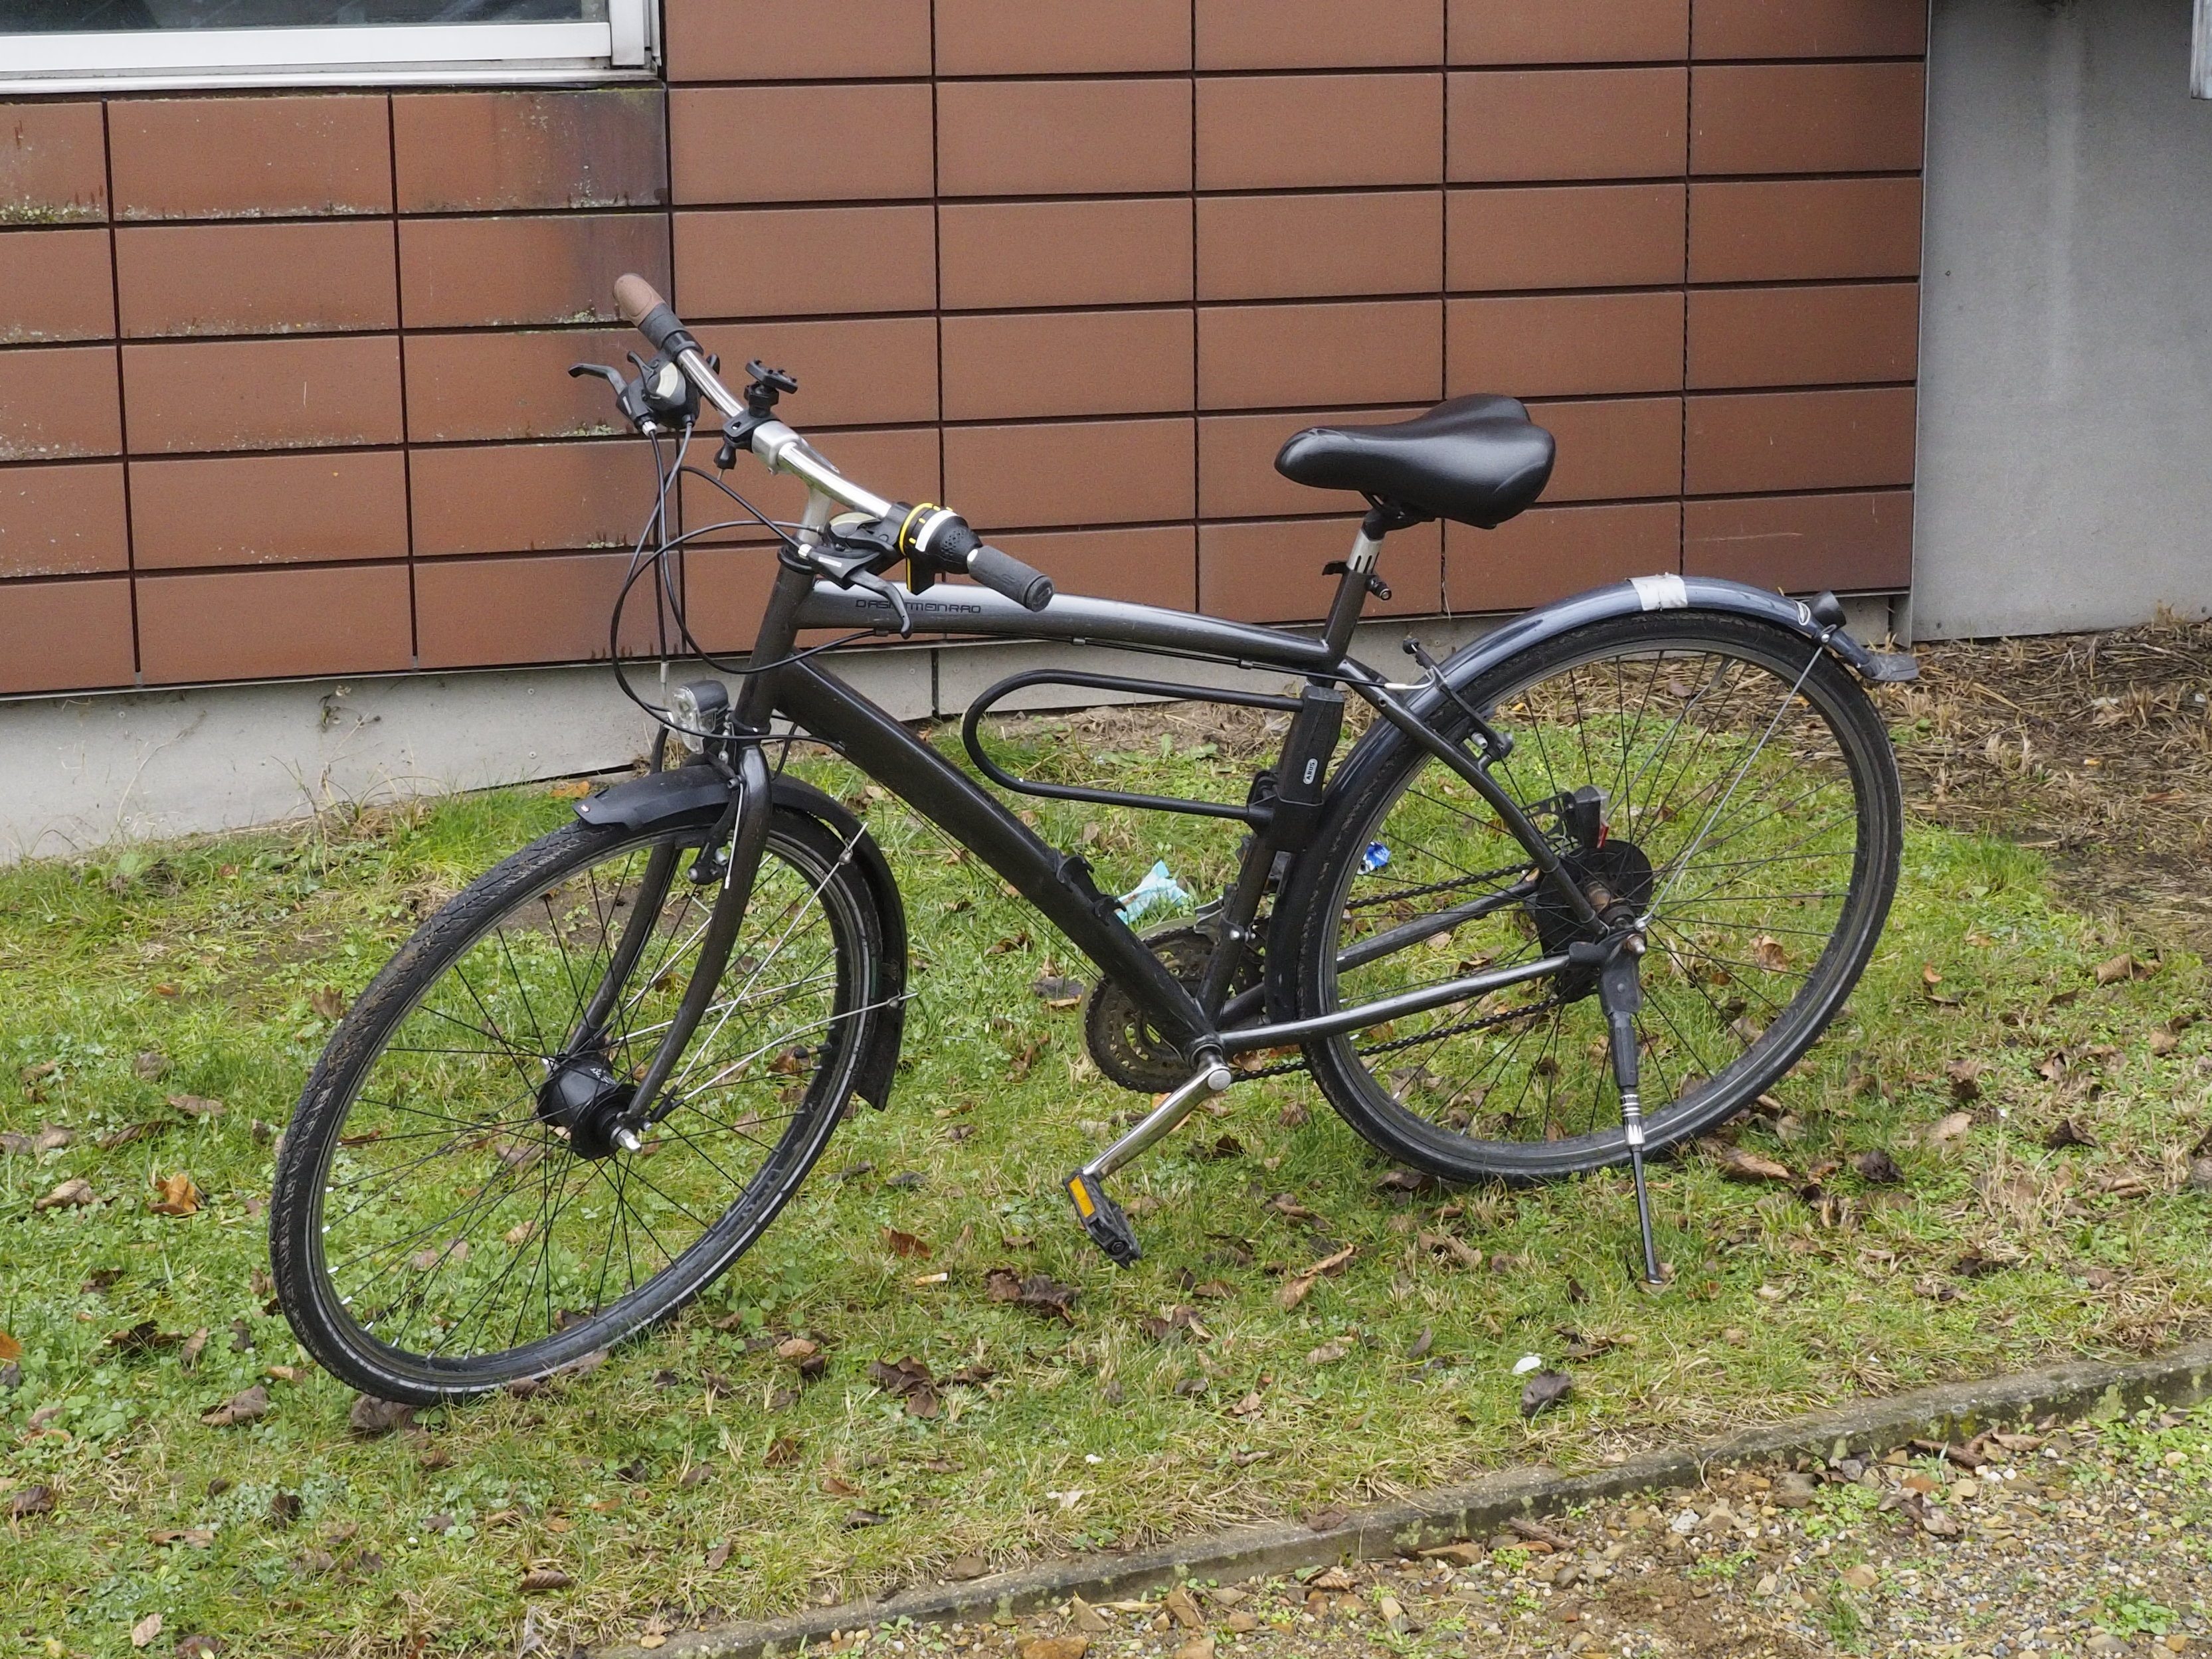
\includegraphics[width=.9413\linewidth]{images/study_bike.jpg}
        \caption{The bicycle used in the field-study}
        \label{fig:study_bike}
    \end{minipage}%
    \begin{minipage}{.4325\textwidth}
        \centering
        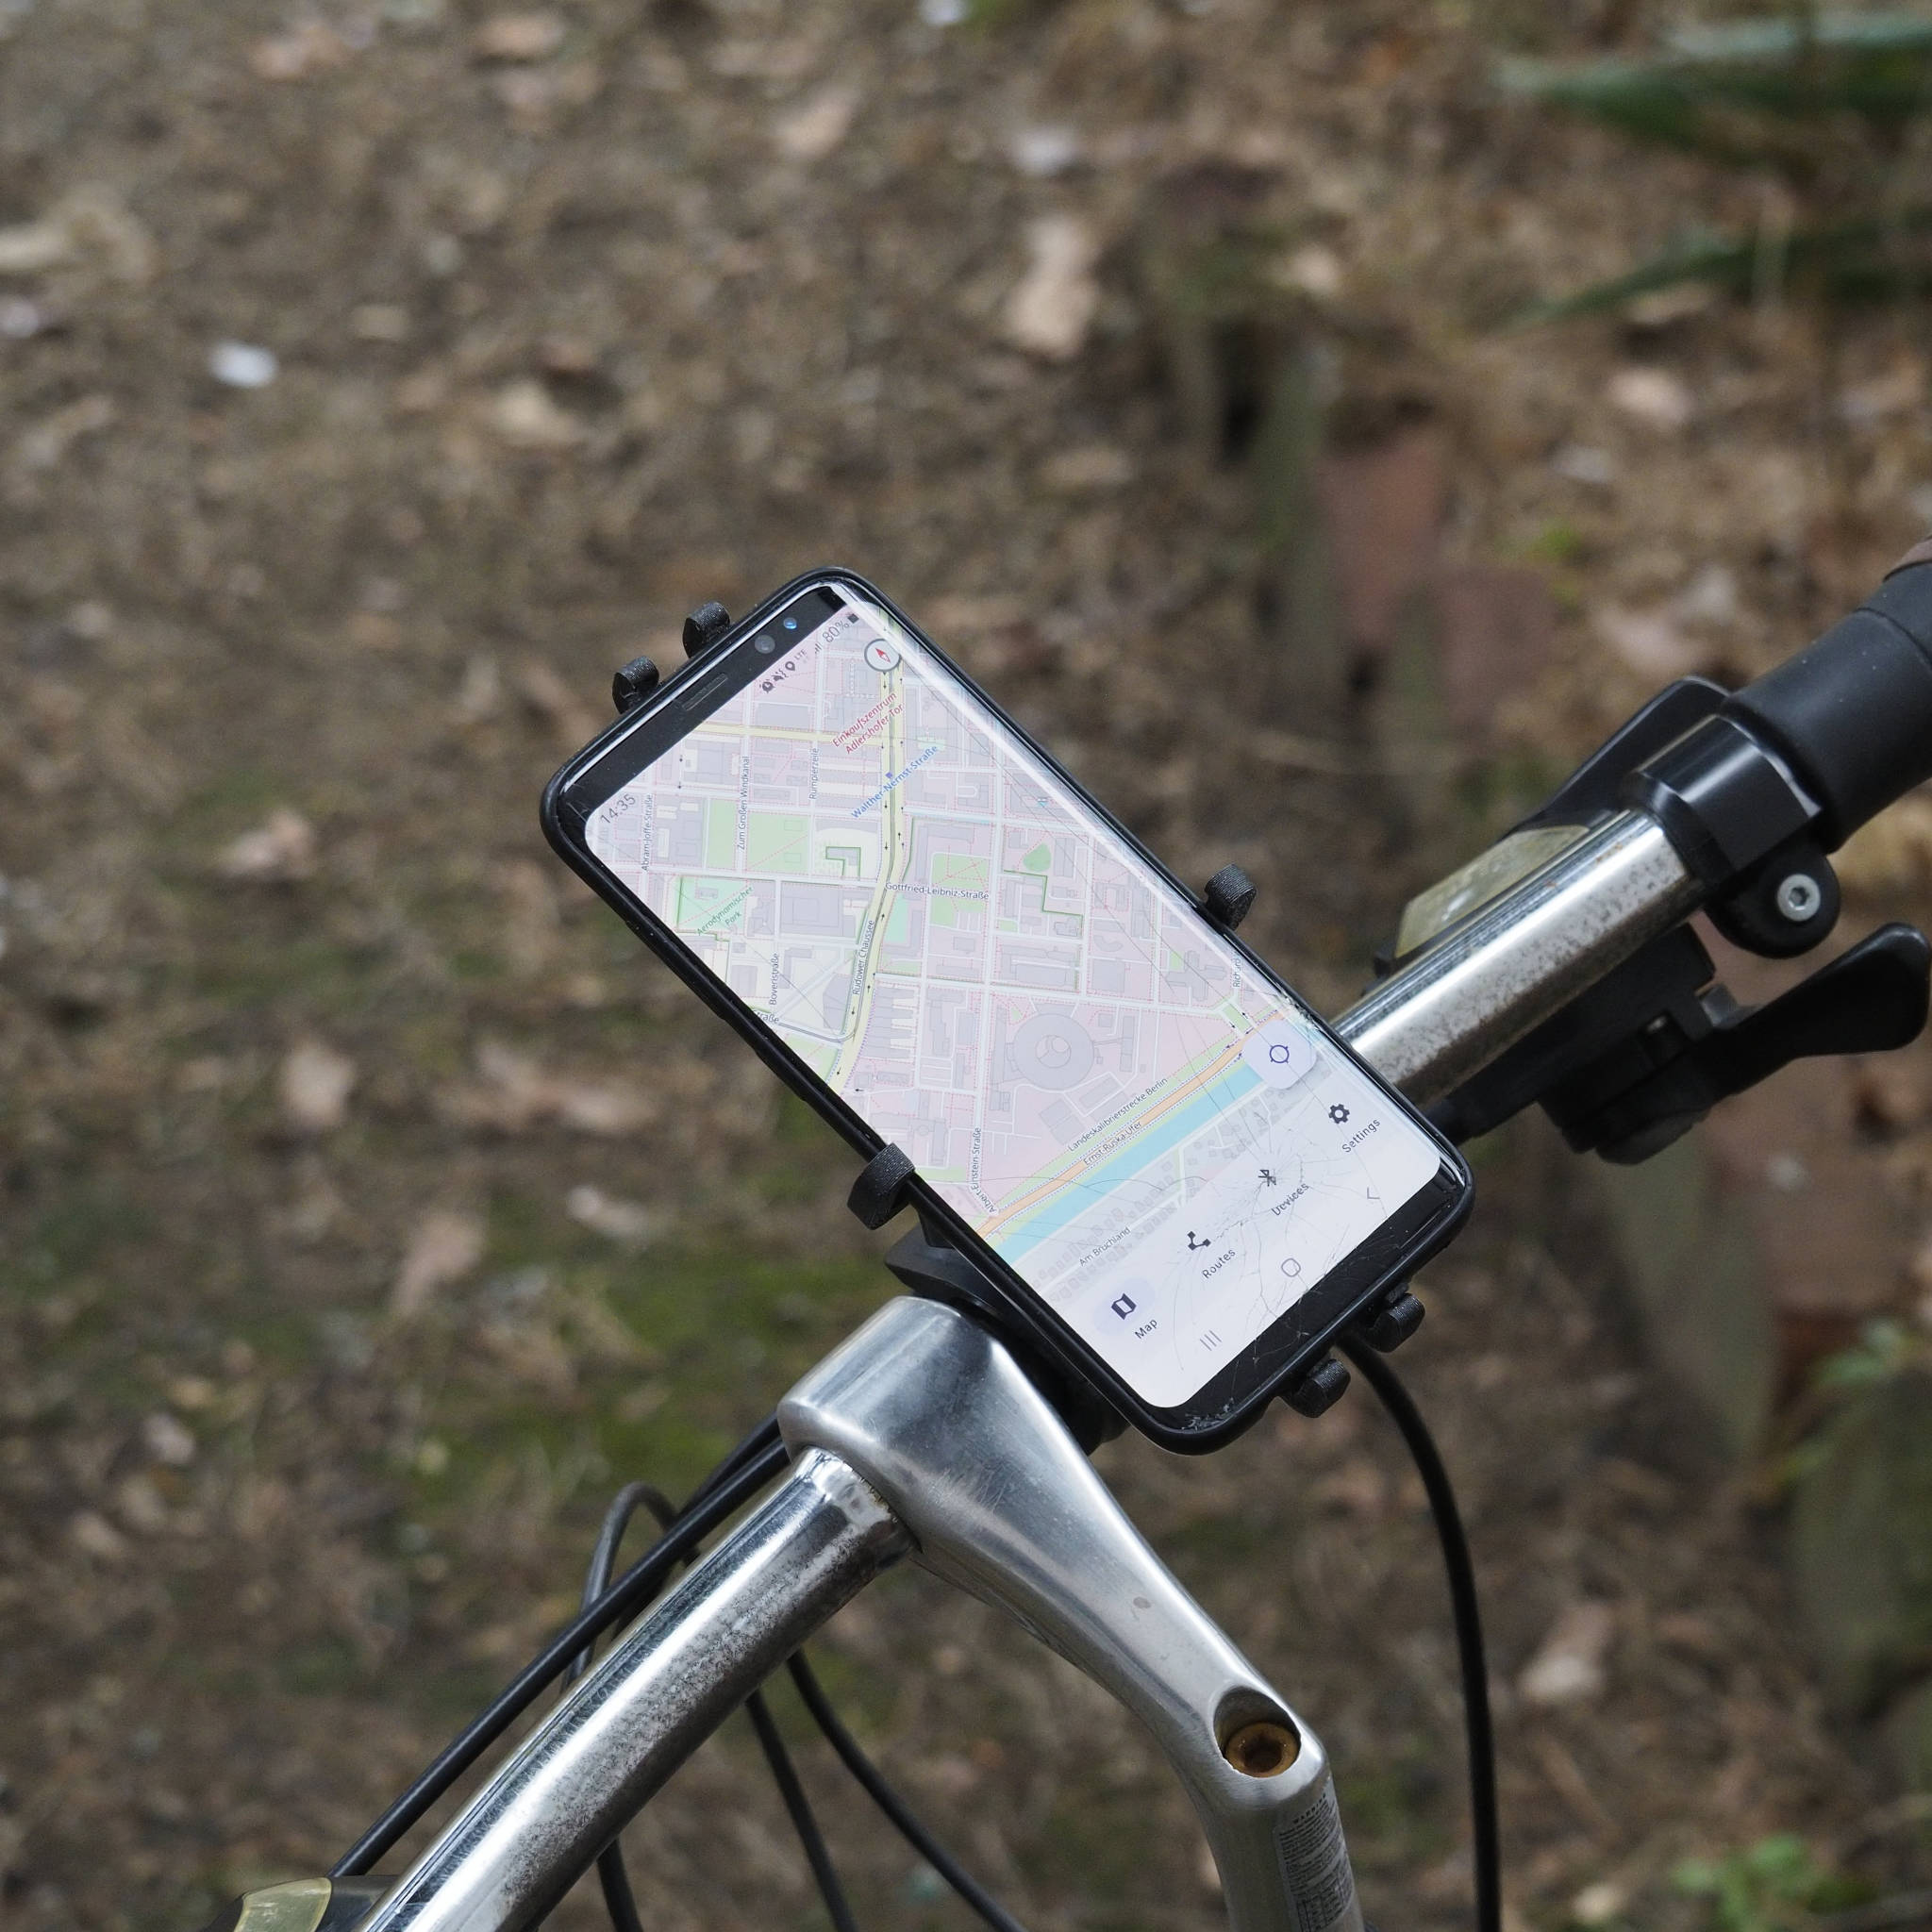
\includegraphics[width=.9229\linewidth]{images/smartphone_holder.jpg}
        \caption{Smartphone holder}
        \label{fig:smartphone_holder}
    \end{minipage}
\end{figure}

\subsubsection*{Safety Precautions}

To ensure each participants' safety, the researcher conducting the study followed them on their routes, retaining a save distance, with another bicycle.
Participants were further told to not look at the route on the smartphone for extended periods of time and to focus their attention on the road in front of them and to stop and get in contact with the researcher if a problem occurred, but to otherwise ignore them.
They were also told to only drive at a conservative, safe speed.
